\chapter{Cypherpunks schreiben Code}
\label{les:20}

\begin{chapquote}{Lewis Carroll, \textit{Alice im Wunderland}}
\enquote{Ich sehe, du versuchst etwas zu erfinden.}
\end{chapquote}

Wie auch viele andere großartige Ideen erschien Bitcoin nicht aus dem Nichts.
Möglich gemacht wurde es durch die Nutzung und Kombination vieler Innovationen
und Entdeckungen in Mathematik, Physik, Informatik und anderen Bereichen. Obwohl
Satoshi zweifellos ein Genie ist, hätte er Bitcoin nicht ohne die Riesen
erfinden können auf deren Schultern er stand.

\begin{quotation}\begin{samepage}
\enquote{Wer nur wünscht und hofft greift nicht aktiv in den Lauf der Dinge und
in die Gestaltung seines eigenen Schicksals ein.}
\begin{flushright} -- Ludwig von Mises\footnote{Ludwig von Mises, \textit{Human
Action} \cite{human-action}}
\end{flushright}\end{samepage}\end{quotation}

Einer dieser Riesen ist Eric Hughes, einer der Gründer der Cypherpunk-Bewegung
und Autor des Cypherpunk-Manifests (\textit{A Cypherpunk's Manifesto}). Es ist
schwer vorstellbar, dass Satoshi nicht von diesem Manifest beeinflusst wurde. Es
spricht von vielen Dingen die Bitcoin ermöglicht und nutzt, wie z.B. direkte und
private Transaktionen, elektronisches Geld und Bargeld, anonyme Systeme und die
Verteidigung der Privatsphäre mit Kryptographie und digitalen Signaturen.

\begin{quotation}\begin{samepage}
\enquote{Datenschutz ist notwendig für eine offene Gesellschaft im
elektronischen Zeitalter. [...] Da wir Privatsphäre anstreben, müssen wir
sicherstellen, dass jede Partei einer Transaktion nur das weiß was für diese
Transaktion direkt notwendig ist. [...] Daher erfordert der Datenschutz in einer
offenen Gesellschaft anonyme Transaktionssysteme. Bislang war Bargeld das
wichtigste derartige System. Ein anonymes Transaktionssystem ist kein geheimes
Transaktionssystem. [...] Wir, die Cypherpunks, widmen uns dem Aufbau anonymer
Systeme. Wir verteidigen unsere Privatsphäre mit Kryptographie, mit anonymen
Mail-Weiterleitungssystemen, mit digitalen Signaturen und mit elektronischem
Geld.

Cypherpunks schreiben Code.}
\begin{flushright} -- Eric Hughes\footnote{Eric Hughes, \textit{A Cypherpunk's Manifesto} \cite{cypherpunk-manifesto}}
\end{flushright}\end{samepage}\end{quotation}

Cypherpunks finden keinen Gefallen an Hoffnungen und Wünschen. Sie greifen aktiv
in den Lauf der Dinge ein und gestalten ihr eigenes Schicksal. Cypherpunks
schreiben Code.

So setzte sich Satoshi in echter Cypherpunk-Manier hin und begann Code zu
schreiben. Code, der eine abstrakte Idee aufnahm und der Welt bewies, dass diese
tatsächlich funktionierte. Code, der den Samen einer neuen wirtschaftlichen
Realität pflanzte. Dank dieses Codes kann jeder überprüfen, ob dieses neuartige
System tatsächlich funktioniert und alle zehn Minuten beweist Bitcoin der Welt,
dass das System am Leben ist.

\begin{figure}
  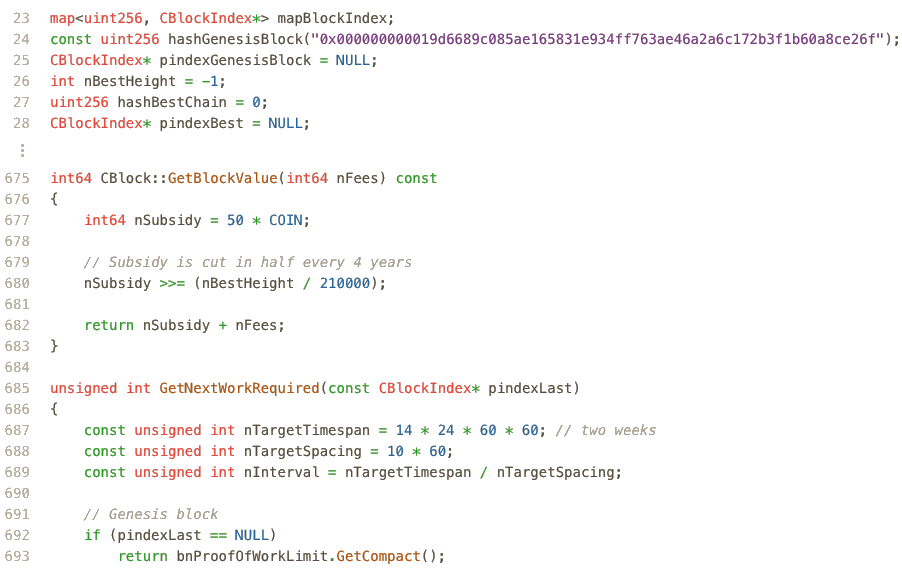
\includegraphics{assets/images/bitcoin-code-white.png}
  \caption{Code-Auszüge aus der Bitcoin Version 0.1}
  \label{fig:bitcoin-code-white}
\end{figure}

Um sicherzustellen dass seine Erfindung die Fantasiephase überwindet und
Wirklichkeit wird, schrieb Satoshi den Code, um seine Idee zu realisieren, noch
bevor er das Whitepaper verfasste. Er achtete auch darauf keine seiner
Veröffentlichungen lange hinauszuzögern\footnote{\enquote{Wir sollten [den
Release] nicht ewig hinauszögern bis jedes Mögliche Feature implementiert ist.}
-- Satoshi Nakamoto~\cite{satoshi-delay}}. Schließlich \enquote{würde es immer
noch etwas zu tun geben}.

\begin{quotation}\begin{samepage}
\enquote{Ich musste zuerst den ganzen Code schreiben bevor ich mich überzeugen konnte, dass ich jedes Problem lösen konnte.
Erst dann schrieb ich das Whitepaper.}
\begin{flushright} -- Satoshi Nakamoto\footnote{Satoshi Nakamoto, \textit{Re: Bitcoin P2P e-cash paper}~\cite{satoshi-mail-code-first}}
\end{flushright}\end{samepage}\end{quotation}

In der heutigen Welt der endlosen Versprechen und fraghaften Umsetzungen, ist die
Implementierung von Bitcoin eine willkommene Abwechslung. Probleme
identifizieren, Lösungswege abwiegen, Lösungen implementieren. Wir sollten alle
darauf hinarbeiten etwas mehr Cypherpunk zu sein.

\paragraph{Bitcoin lehrte mich, dass Cypherpunks Code schreiben.}

% ---
%
% #### Down the Rabbit Hole
%
% - [Bitcoin version 0.1.0 announcement][version 0.1.0] by Satoshi Nakamoto
% - [Bitcoin P2P e-cash paper announcement][mail-announcement] by Satoshi Nakamoto
%
% [mail-announcement]: http://www.metzdowd.com/pipermail/cryptography/2008-October/014810.html
% [Ludwig Von Mises]: https://mises.org/library/human-action-0/html/pp/613
% [version 0.1.0]: https://bitcointalk.org/index.php?topic=68121.0
% [not to delay]: https://bitcointalk.org/index.php?topic=199.msg1670#msg1670
% [6]: http://www.metzdowd.com/pipermail/cryptography/2008-November/014832.html
%
% <!-- Wikipedia -->
% [alice]: https://en.wikipedia.org/wiki/Alice%27s_Adventures_in_Wonderland
% [carroll]: https://en.wikipedia.org/wiki/Lewis_Carroll
